\documentclass[12pt,a4paper]{article}
\usepackage[utf8]{inputenc}
\usepackage{geometry}
\geometry{a4paper, margin=1in}
\usepackage{graphicx}
\usepackage{amsmath}
\usepackage{hyperref}
\usepackage{listings}
\usepackage{xcolor}
\usepackage{tocloft}
\usepackage{tikz}
\usetikzlibrary{shapes.geometric, arrows, positioning}

% Ensure section dot leaders in Table of Contents to match screenshot
\renewcommand{\cftsecleader}{\cftdotfill{\cftdotsep}}

% Custom Colors matching screenshots
\definecolor{univcolor}{HTML}{A0522D} % Sienna / Brown-Orange for University Name
\definecolor{titlecolor}{HTML}{0000FF} % Bright Blue for titles

\definecolor{dkgreen}{rgb}{0,0.6,0}
\definecolor{gray}{rgb}{0.5,0.5,0.5}
\definecolor{mauve}{rgb}{0.58,0,0.82}

\lstset{frame=tb,
  language=SQL,
  aboveskip=3mm,
  belowskip=3mm,
  showstringspaces=false,
  columns=flexible,
  basicstyle={\small\ttfamily},
  numbers=none,
  numberstyle=\tiny\color{gray},
  keywordstyle=\color{blue},
  commentstyle=\color{dkgreen},
  stringstyle=\color{mauve},
  breaklines=true,
  breakatwhitespace=true,
  tabsize=3
}

\begin{document}

% ==========================================
% COVER PAGE (Screenshot 1)
% ==========================================
\begin{titlepage}
    \begin{center}
        \Large
        \textcolor{univcolor}{\textbf{TEZPUR UNIVERSITY}}
        
        \vspace{0.8cm}
        
        % Logo matching screenshot
        \includegraphics[width=3.5cm,keepaspectratio]{tezpur_logo.png}
        
        \vspace{0.8cm}
        
        \large
        \textbf{BACHELOR OF TECHNOLOGY} \\
        COMPUTER SCIENCE \& ENGINEERING
        
        \vspace{1.5cm}
        
        \normalsize
        \textbf{Project Report on} \\
        \vspace{0.3cm}
        \Large
        \textcolor{titlecolor}{\textbf{TU HOSTEL COMPLAINT MANAGEMENT SYSTEM}}
        
        \vspace{2.0cm}
        
        \normalsize
        \textit{Submitted By} \\
        \vspace{0.2cm}
        \large
        \textbf{SPANDAN SARMA, CSB23075} \\
        \textbf{YAJANT NATH TRIPATHI, CSB23072}
        
        \vspace{1.5cm}
        
        \normalsize
        \textit{Under the guidance of} \\
        \vspace{0.2cm}
        \large
        \textbf{DR. JYOTISMITA TALUKDAR} \\
        \normalsize
        Department of Computer Science \& Engineering \\
        \vspace{0.2cm}
        \large
        \textbf{6TH SEMESTER / 2026}
        
        \vfill
        
        \small
        \textcolor{titlecolor}{\textbf{DEPARTMENT OF COMPUTER SCIENCE \& ENGINEERING}} \\
        \textcolor{titlecolor}{\textbf{TEZPUR UNIVERSITY, ASSAM, 784028}}
        
    \end{center}
\end{titlepage}

% ==========================================
% CERTIFICATE PAGE (Screenshot 2)
% ==========================================
\newpage
\thispagestyle{plain}
\begin{center}
    \large
    \textcolor{univcolor}{\textbf{Tezpur University}} \\
    \small \textcolor{univcolor}{Napaam, Tezpur, Assam - 784028}
\end{center}

\noindent
\Large \textcolor{titlecolor}{\textbf{Department of Computer Science \& Engineering}}

\vspace{1cm}
\begin{center}
    \large
    \textbf{\underline{CERTIFICATE}}
\end{center}

\vspace{0.5cm}
\noindent
\normalsize
This is to certify that the project report entitled \textbf{``TU Hostel Complaint Management System''} is a genuine record of student work carried out under guidance by \textbf{Spandan Sarma (Roll No. CSB23075)} and \textbf{Yajant Nath Tripathi (Roll No. CSB23072)}. The contents of this report have not been submitted elsewhere for any academic degree or diploma.

\vspace{2cm}
\noindent
\begin{tabular*}{\textwidth}{@{\extracolsep{\hfill}}lll@{}}
\textbf{GUIDE DETAILS} & \textbf{COORDINATOR DETAILS} & \textbf{HOD DETAILS} \\
Dr. Jyotismita Talukdar & Prof. Priya Sharma & Prof. Bhabesh Nath \\[1.2cm]
Signature: ......................... & Signature: ......................... & Signature: .........................
\end{tabular*}

\vspace{2.5cm}
\noindent
\textbf{Name of Examiners:} \hfill \textbf{Signature with Date:}
\vspace{0.6cm}

\noindent
1. \rule{6.5cm}{0.4pt} \hfill \rule{6.5cm}{0.4pt} \\[0.8cm]
2. \rule{6.5cm}{0.4pt} \hfill \rule{6.5cm}{0.4pt} \\[0.8cm]
3. \rule{6.5cm}{0.4pt} \hfill \rule{6.5cm}{0.4pt}

% ==========================================
% ACKNOWLEDGEMENT PAGE (Screenshot 3)
% ==========================================
\newpage
\begin{center}
    \Large \textbf{\underline{Acknowledgement}}
\end{center}

\vspace{1cm}
\noindent
We would like to express our sincere appreciation to our project guide, Dr. Jyotismita Talukdar, for her support and insights. We also thank the Department of Computer Science \& Engineering at Tezpur University for providing access to development environments and servers necessary to carry out this project.

We are also grateful to our peers and the hostel office staff who participated in interviews and user testing, helping us align the system workflows with real-world requirements.

\vspace{2cm}
\noindent
\textbf{SPANDAN SARMA (CSB23075)} \\
\textbf{YAJANT NATH TRIPATHI (CSB23072)}

% ==========================================
% ABSTRACT PAGE (Screenshot 4)
% ==========================================
\newpage
\begin{center}
    \Large \textbf{\underline{Abstract}}
\end{center}

\vspace{1cm}
\noindent
Hostel administration represents a critical component of university infrastructure, directly impacting the well-being and academic performance of resident students. In many institutions, including Tezpur University, utility and infrastructure complaints (such as plumbing, electricity, carpentry, and internet maintenance) are managed via manual, paper-based registers. This operational approach introduces significant bottlenecks, including slow response times, absence of ticket progress visibility, lack of administrative accountability, and no structured escalation paths when repairs are delayed.

To address these limitations, this project presents the \textbf{TU Hostel Complaint Management System} (also known as \textit{DormFix}), an enterprise-grade web-based solution. The system replaces fragmented paper records with a unified database workflow, managing the entire lifecycle of a complaint. Built on a tech stack of \textbf{Next.js} (TypeScript) for the frontend, \textbf{Express/Node.js} for the backend scaffold, and a \textbf{PostgreSQL} relational database, the system enforces role-based workflows across five specialized user interfaces: Student, Warden, Maintenance Department, Dean of Student Welfare (DSW), and Vice Chancellor (VC).

The system integrates a \textbf{Shared Institutional Clock} and \textbf{SLA (Service Level Agreement) Engine} that enforces strict deadlines based on issue urgency (Critical: 6h, High: 24h, Medium: 48h, Low: 72h). If a deadline is breached, the ticket is escalated to higher authorities (Warden $\rightarrow$ DSW $\rightarrow$ VC). To ensure high-quality repairs, the system requires multi-stage digital evidence handovers: students upload photos of the initial damage, maintenance staff upload technical verification photos of the fix, and wardens submit final checks. A real-time analytics module on the VC dashboard compiles response times and resolution statistics, providing data-driven tools for institutional management.

% ==========================================
% CONTENTS PAGE (Screenshot 5)
% ==========================================
\newpage
\tableofcontents

% ==========================================
% 1. INTRODUCTION (Screenshot 6)
% ==========================================
\newpage
\section{Introduction}

\subsection{Scope}
The scope of the TU Hostel Complaint Management System is focused on digitizing, monitoring, and auditing utility and structural maintenance complaints within the residential hostels of Tezpur University. The system is designed to coordinate operations across 12 active student hostels, accommodating over 4,000 residents. The platform strictly targets utility domains including Plumbing, Electrical, IT Support, Carpentry, Housekeeping, and General Maintenance. 

Academic disputes, disciplinary records, mess menu adjustments, and general student welfare issues fall outside the system boundary. The application coordinates roles from the student filing a complaint, to the warden approving and routing the request, the specific maintenance cell executing the repair, the DSW monitoring breaches, and the Vice Chancellor auditing campus-wide infrastructure health.

\subsection{Purpose of the Project}
The primary purpose of the project is to replace slow, paper-based hostel complaint logs with an automated digital workflow. Under the manual register system, complaints are frequently neglected due to a lack of tracking, leading to student frustration. The digital system introduces a Shared Institutional Clock that starts the moment a student submits a ticket. 

By binding maintenance operations to a Service Level Agreement (SLA), the system makes response times visible, holds maintenance cells accountable, and provides a clear mechanism for escalation. The project also introduces photographic verification requirements to build a transparent, evidence-backed chain of custody, ensuring that repair work is completed to standard.

\subsection{Overview of the Report}
This report documents the design, architecture, and implementation of the Hostel Complaint Management System. Section 2 outlines the problem statement and the inefficiencies of the manual system. Section 3 details the Software Requirements Specification (SRS), focusing on functional, non-functional, and system constraints. Section 4 presents the Data Flow Diagrams (DFDs) at Levels 0 and 1. 

Section 5 describes the system objectives. Section 6 presents the feasibility study. Section 7 details the three-tier system architecture and interaction sequences. Section 8 displays the detailed flowchart of the ticket lifecycle. Section 9 outlines the database and directory structures. Section 10 describes the features implemented in the dashboards. Finally, Sections 11 through 15 present limitations, future scope, conclusions, references, and appendices.

% ==========================================
% 2. PROBLEM STATEMENT (Screenshot 7)
% ==========================================
\newpage
\section{Problem Statement}
Tezpur University maintains multiple student hostels spread across its campus. Each hostel currently manages utility maintenance requests using physical paper registers located in the common lobbies. This manual operational model introduces several critical issues:
\begin{itemize}
    \item \textbf{No Real-Time Visibility:} Students have no way to track their filed complaints. They must repeatedly check with the hostel office or warden to see if a technician has been contacted.
    \item \textbf{Absence of Maintenance Accountability:} Maintenance wings (Electrical, IT support, Plumbing) operate without performance tracking. There are no metrics to measure how long a department takes to respond to and resolve complaints.
    \item \textbf{No Escalation for Delays:} If a critical complaint (such as a water pump failure or power outage) is delayed by days, there is no automatic system to notify the warden, the DSW, or the VC. This results in prolonged utility outages.
    \item \textbf{Lack of Verification:} In the paper system, a complaint is marked resolved based on verbal updates from the technician. This often leads to incomplete repairs without any quality check.
\end{itemize}
To resolve these issues, the university requires a digital, role-based platform that tracks complaints in real-time, enforces resolution deadlines, and verifies repairs using photographic evidence.

% ==========================================
% 3. SRS (Screenshot 8)
% ==========================================
\newpage
\section{Software Requirements Specification (SRS)}

\subsection{Functional Requirements}
\begin{itemize}
    \item \textbf{FR-1 (Secure Authentication):} The system must authenticate users via secure login screens and direct them to their role-specific dashboard (Student, Warden, Department, DSW, or VC).
    \item \textbf{FR-2 (Complaint Filing):} Students must be able to submit maintenance tickets by entering the title, description, location (pre-bound to their room), urgency level, and uploading photos of the issue.
    \item \textbf{FR-3 (Warden Routing):} Wardens must have an interface to review pending complaints within their hostel and assign them to the appropriate maintenance department (e.g. Electrical, Plumbing).
    \item \textbf{FR-4 (Departmental Worklist):} Department heads must be able to view assigned tickets, transition status from \texttt{filed} to \texttt{in\_progress}, upload verification photos of the repair, and mark them \texttt{resolved}.
    \item \textbf{FR-5 (Automated Escalation):} The system must track SLA countdowns and automatically mark tickets as \texttt{escalated} if they exceed the allocated resolution window.
    \item \textbf{FR-6 (Administrative Auditing):} The VC and DSW must be able to view campus-wide metrics, including average resolution times and department efficiency.
\end{itemize}

\subsection{Non-Functional Requirements}
\begin{itemize}
    \item \textbf{Performance:} The web interface must load dashboards within 1.5 seconds, even under peak load conditions.
    \item \textbf{Usability:} The UI must be fully responsive, adapting to mobile, tablet, and desktop viewports to support technicians on-site.
    \item \textbf{Security:} Passwords must be hashed using bcrypt before database storage. Express API routes must be protected using JWT tokens.
    \item \textbf{Data Integrity:} Database interactions must use transaction locks to prevent race conditions during status updates.
\end{itemize}

\subsection{System Requirements}
\begin{itemize}
    \item \textbf{Server OS:} Linux (Ubuntu Server 20.04 LTS or newer recommended) or Windows Server.
    \item \textbf{Database System:} PostgreSQL 14 or higher.
    \item \textbf{Development Runtime:} Node.js v18.0.0 or higher.
    \item \textbf{Frontend Libraries:} Next.js 14, Tailwind CSS, Lucide React, and shadcn/ui.
    \item \textbf{Backend Scaffold:} Express framework with TypeScript compilation.
\end{itemize}

% ==========================================
% 4. DFD (Screenshots 9 & 10)
% ==========================================
\newpage
\section{Data Flow Diagrams (DFD)}

\subsection{Level 0 DFD}
The Level 0 Context Data Flow Diagram defines the boundary of the system, illustrating how the external entities (Student, Warden, Department, DSW, and VC) interact with the central application.

\begin{figure}[h!]
\centering
\setlength{\fboxsep}{10pt}
\fbox{
    \begin{minipage}[c][11.5cm][c]{0.95\textwidth}
        \centering
        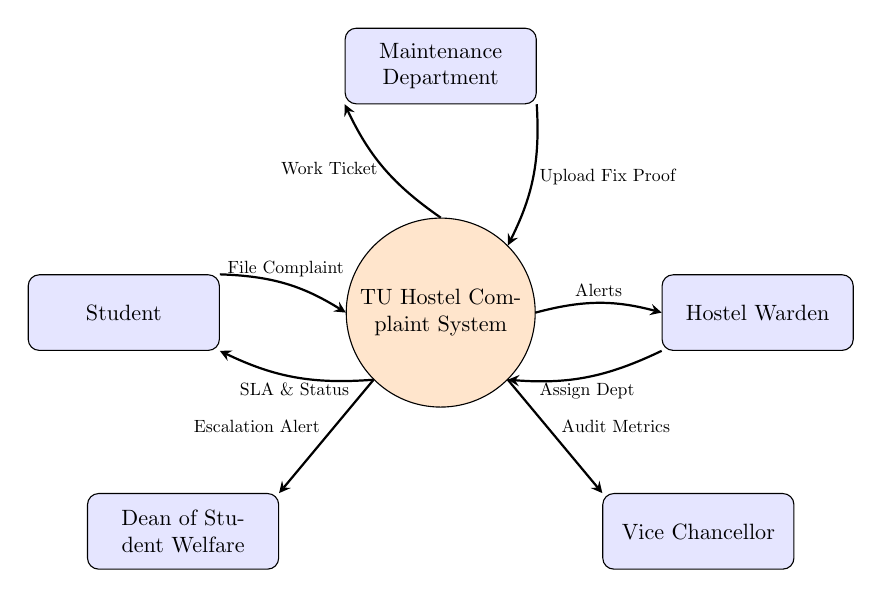
\begin{tikzpicture}[scale=0.8, every node/.style={transform shape},
            block/.style={draw, rectangle, rounded corners, minimum width=3cm, minimum height=1.2cm, text centered, draw=black, fill=blue!10, text width=2.8cm},
            process/.style={draw, circle, minimum size=3cm, text centered, draw=black, fill=orange!20, text width=2.6cm},
            arrow/.style={thick,->,>=stealth}]
            
            % Nodes
            \node (system) [process] {TU Hostel Complaint System};
            \node (student) [block, left=of system, xshift=-1cm] {Student};
            \node (warden) [block, right=of system, xshift=1cm] {Hostel Warden};
            \node (dept) [block, above=of system, yshift=0.8cm] {Maintenance Department};
            \node (dsw) [block, below left=of system, xshift=-0.5cm, yshift=-0.8cm] {Dean of Student Welfare};
            \node (vc) [block, below right=of system, xshift=0.5cm, yshift=-0.8cm] {Vice Chancellor};

            % Arrows
            % Student <-> System
            \draw [arrow] (student.north east) to [bend left=15] node[above, scale=0.8] {File Complaint} (system.west);
            \draw [arrow] (system.south west) to [bend left=15] node[below, scale=0.8] {SLA \& Status} (student.south east);
            
            % Warden <-> System
            \draw [arrow] (system.east) to [bend left=15] node[above, scale=0.8] {Alerts} (warden.west);
            \draw [arrow] (warden.south west) to [bend left=15] node[below, scale=0.8] {Assign Dept} (system.south east);
            
            % Dept <-> System
            \draw [arrow] (system.north) to [bend left=15] node[left, scale=0.8] {Work Ticket} (dept.south west);
            \draw [arrow] (dept.south east) to [bend left=15] node[right, scale=0.8] {Upload Fix Proof} (system.north east);
            
            % System -> DSW
            \draw [arrow] (system.south west) to node[left, scale=0.8, yshift=0.2cm] {Escalation Alert} (dsw.north east);
            
            % System -> VC
            \draw [arrow] (system.south east) to node[right, scale=0.8, yshift=0.2cm] {Audit Metrics} (vc.north west);
        \end{tikzpicture}
    \end{minipage}
}
\caption{Level 0 Data Flow Diagram}
\end{figure}

\newpage
\subsection{Level 1 DFD}
The Level 1 Data Flow Diagram breaks the system down into its primary sub-processes, displaying how data is queried and modified within the database tables during key transitions.

\begin{figure}[h!]
\centering
\setlength{\fboxsep}{10pt}
\fbox{
    \begin{minipage}[c][13.5cm][c]{0.95\textwidth}
        \centering
        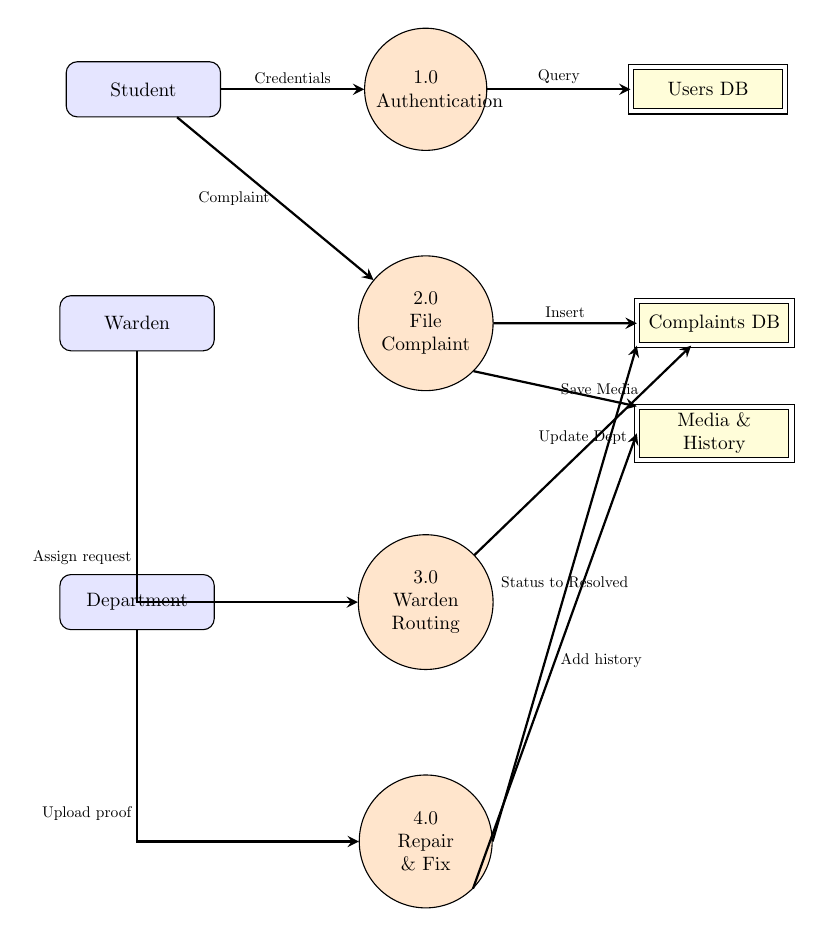
\begin{tikzpicture}[scale=0.7, every node/.style={transform shape},
            node distance=1.4cm,
            block/.style={draw, rectangle, rounded corners, minimum width=2.8cm, minimum height=1.0cm, text centered, draw=black, fill=blue!10, text width=2.5cm},
            process/.style={draw, circle, minimum size=2cm, text centered, draw=black, fill=orange!20, text width=1.8cm},
            datastore/.style={draw, rectangle, minimum width=2.8cm, minimum height=0.8cm, text centered, draw=black, fill=yellow!15, double distance=1.5pt, text width=2.4cm},
            arrow/.style={thick,->,>=stealth}]
            
            % Row 1
            \node (student) [block] {Student};
            \node (p1) [process, right=of student, xshift=1.2cm] {1.0\\Authentication};
            \node (db_users) [datastore, right=of p1, xshift=1.2cm] {Users DB};
            
            % Row 2
            \node (p2) [process, below=of p1, yshift=-0.5cm] {2.0\\File Complaint};
            \node (db_complaints) [datastore, right=of p2, xshift=1.2cm] {Complaints DB};
            \node (db_media) [datastore, below=of db_complaints, yshift=0.3cm] {Media \& History};
            
            % Row 3
            \node (warden) [block, left=of p2, xshift=-1.2cm] {Warden};
            \node (p3) [process, below=of p2, yshift=-1.2cm] {3.0\\Warden Routing};
            
            % Row 4
            \node (dept) [block, left=of p3, xshift=-1.2cm] {Department};
            \node (p4) [process, below=of p3, yshift=-0.5cm] {4.0\\Repair \& Fix};

            % Connections
            \draw [arrow] (student) -- node[above, scale=0.8] {Credentials} (p1);
            \draw [arrow] (p1) -- node[above, scale=0.8] {Query} (db_users);
            \draw [arrow] (student) -- node[left, scale=0.8] {Complaint} (p2);
            \draw [arrow] (p2) -- node[above, scale=0.8] {Insert} (db_complaints);
            \draw [arrow] (p2.south east) -- node[right, scale=0.8] {Save Media} (db_media.north west);
            
            \draw [arrow] (warden) |- node[left, yshift=0.8cm, scale=0.8] {Assign request} (p3);
            \draw [arrow] (p3) -- node[above, scale=0.8] {Update Dept} (db_complaints);
            
            \draw [arrow] (dept) |- node[left, yshift=0.5cm, scale=0.8] {Upload proof} (p4);
            \draw [arrow] (p4.east) -- node[above, scale=0.8] {Status to Resolved} (db_complaints.south west);
            \draw [arrow] (p4.south east) -- node[right, scale=0.8] {Add history} (db_media.west);
        \end{tikzpicture}
    \end{minipage}
}
\caption{Level 1 Data Flow Diagram}
\end{figure}

% ==========================================
% 5. OBJECTIVES (Screenshot 11)
% ==========================================
\newpage
\section{Objectives}
The core objectives of the TU Hostel Complaint Management System are structured to optimize communication, enforce accountability, and establish transparency within residential facilities:
\begin{enumerate}
    \item \textbf{Enforce Strict SLAs:}
    \begin{itemize}
        \item Establish clear resolution windows based on issue urgency: Critical (6 hours), High (24 hours), Medium (48 hours), and Low (72 hours) to minimize delays for essential utilities.
    \end{itemize}
    \item \textbf{Provide Transparent Progress Logs:}
    \begin{itemize}
        \item Maintain a complete transaction history in the database (\texttt{complaint\_history}) so students can view who accepted their ticket and when changes occurred.
    \end{itemize}
    \item \textbf{Require Photographic Verification:}
    \begin{itemize}
        \item Enforce a policy requiring technicians to upload a photo of the completed repair before a ticket can be set to resolved, preventing premature closures.
    \end{itemize}
    \item \textbf{Automate Escalation Paths:}
    \begin{itemize}
        \item Automatically escalate delayed complaints to the DSW and VC dashboards, ensuring administration can identify backlogs.
    \end{itemize}
\end{enumerate}

% ==========================================
% 6. FEASIBILITY STUDY (Screenshot 12)
% ==========================================
\newpage
\section{Feasibility Study}
A multidimensional feasibility study was conducted to evaluate the viability of deploying the digital platform at Tezpur University:
\begin{enumerate}
    \item \textbf{Technical Feasibility}
    \begin{itemize}
        \item Next.js App Router and PostgreSQL are suitable for this application. PostgreSQL handles relational integrity and transactions, while Next.js server components handle API queries efficiently. The developer team has the required web development skills.
    \end{itemize}
    \item \textbf{Economic Feasibility}
    \begin{itemize}
        \item The platform is built using open-source tools (Node.js, PostgreSQL, Tailwind), which avoids software licensing costs. It can be hosted on existing university servers, keeping deployment and maintenance costs low.
    \end{itemize}
    \item \textbf{Operational Feasibility}
    \begin{itemize}
        \item The system is designed with a user-friendly layout for students and staff. Technicians can access their task list on mobile devices while working on-site, and the automated routing reduces warden administrative overhead, supporting high system adoption.
    \end{itemize}
\end{enumerate}

% ==========================================
% 7. SYSTEM ARCHITECTURE (Screenshot 13)
% ==========================================
\newpage
\section{System Architecture}

\subsection{Subsystems and Components}
The platform uses a three-tier software architecture to separate concerns, improve security, and simplify maintenance:
\begin{itemize}
    \item \textbf{Presentation Layer (UI Client):} Built using Next.js with TypeScript. Tailwind CSS handles styling, and shadcn/ui components provide an interactive dashboard layout for all five user roles.
    \item \textbf{Application Logic Layer (API Router):} Express routing controllers process user requests, handle authentication, validate input data, process image uploads, and calculate SLA deadlines.
    \item \textbf{Data Access Layer (PostgreSQL):} A relational database that stores system records and enforces foreign key constraints across users, hostels, departments, complaints, history, and media tables.
\end{itemize}

\subsection{Interaction Flow}
When a student submits a complaint, the application calculates the escalation deadline based on the selected urgency level and creates a record in the database. The warden receives a notification on their dashboard and assigns the ticket to a maintenance department (e.g., Electrical). 

The department head receives the task, assigns a technician, and updates the status to \texttt{in\_progress}. Once the repair is complete, the technician uploads photographic proof of the fix and marks the ticket as resolved. If a department misses the deadline, a database trigger or scheduler updates the status to \texttt{escalated}, notifying the DSW and VC.

% ==========================================
% 8. DETAILED FLOWCHARTS (Screenshot 14)
% ==========================================
\newpage
\section{Detailed Flowcharts}

\subsection{Flowchart Title}
The flowchart below illustrates the lifecycle of a complaint, mapping all possible states and decision checks from submission to final closure.

\begin{figure}[h!]
\centering
\setlength{\fboxsep}{10pt}
\fbox{
    \begin{minipage}[c][15.5cm][c]{0.95\textwidth}
        \centering
        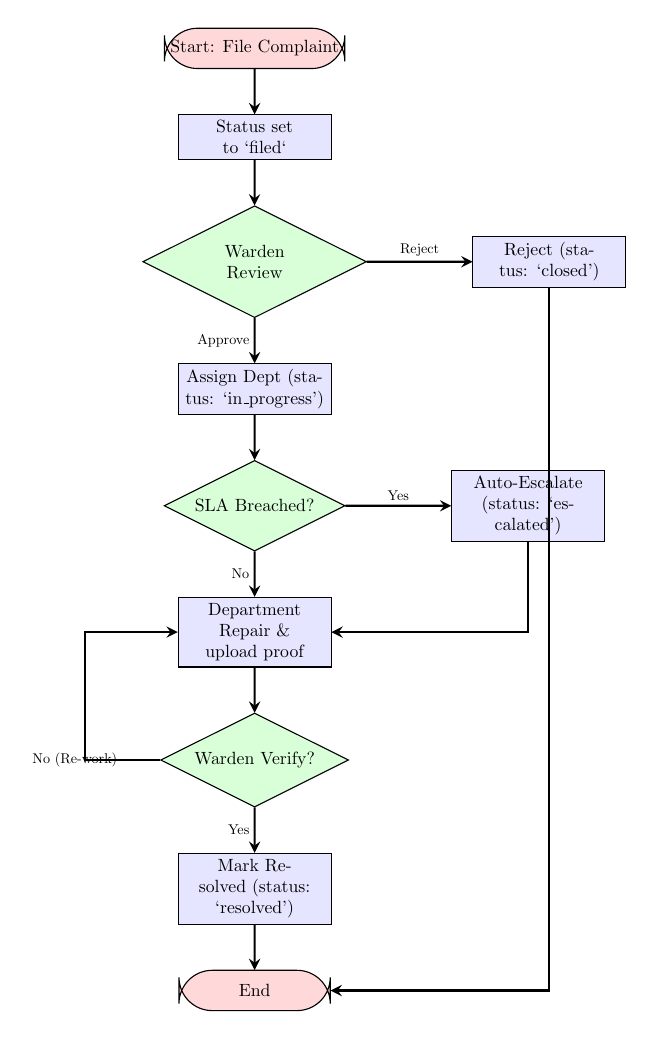
\begin{tikzpicture}[scale=0.64, every node/.style={transform shape},
            node distance=0.9cm,
            startstop/.style={draw, rectangle, rounded corners=12pt, minimum width=3cm, minimum height=0.8cm, text centered, draw=black, fill=red!15},
            process/.style={draw, rectangle, minimum width=3cm, minimum height=0.8cm, text centered, draw=black, fill=blue!10, text width=2.8cm},
            decision/.style={draw, diamond, aspect=2, minimum width=3cm, minimum height=0.8cm, text centered, draw=black, fill=green!15, text width=2.4cm},
            arrow/.style={thick,->,>=stealth}]
            
            % Nodes
            \node (start) [startstop] {Start: File Complaint};
            \node (filed) [process, below=of start] {Status set to `filed`};
            \node (warden) [decision, below=of filed] {Warden Review};
            \node (reject) [process, right=of warden, xshift=1.2cm] {Reject (status: `closed')};
            \node (assign) [process, below=of warden] {Assign Dept (status: `in\_progress')};
            \node (sla) [decision, below=of assign] {SLA Breached?};
            \node (escalate) [process, right=of sla, xshift=1.2cm] {Auto-Escalate (status: `escalated')};
            \node (work) [process, below=of sla] {Department Repair \& upload proof};
            \node (verify) [decision, below=of work] {Warden Verify?};
            \node (resolved) [process, below=of verify] {Mark Resolved (status: `resolved')};
            \node (end) [startstop, below=of resolved] {End};

            % Arrows
            \draw [arrow] (start) -- (filed);
            \draw [arrow] (filed) -- (warden);
            \draw [arrow] (warden) -- node[above, scale=0.8] {Reject} (reject);
            \draw [arrow] (warden) -- node[left, scale=0.8] {Approve} (assign);
            \draw [arrow] (assign) -- (sla);
            \draw [arrow] (sla) -- node[above, scale=0.8] {Yes} (escalate);
            \draw [arrow] (sla) -- node[left, scale=0.8] {No} (work);
            \draw [arrow] (work) -- (verify);
            \draw [arrow] (verify.west) -- node[left, scale=0.8] {No (Re-work)} ++(-1.5cm,0) |- (work.west);
            \draw [arrow] (verify) -- node[left, scale=0.8] {Yes} (resolved);
            \draw [arrow] (resolved) -- (end);
            \draw [arrow] (reject) |- (end);
            \draw [arrow] (escalate) |- (work);
        \end{tikzpicture}
    \end{minipage}
}
\caption{Complaint Lifecycle Flowchart}
\end{figure}

% ==========================================
% 9. CODE STRUCTURE (Screenshot 15)
% ==========================================
\newpage
\section{Code Structure}
The repository is structured as a monorepo containing a frontend and a backend codebase. Below is an overview of the key directories and their functions:
\begin{itemize}
    \item \textbf{frontend/app/api}: Handles Next.js API routes (e.g. auth, complaints, departments, hostels, upload). These routes connect directly to the database.
    \item \textbf{frontend/components}: Manages user interfaces, including dashboards for students, wardens, departments, DSW, and the VC.
    \item \textbf{frontend/lib/db}: Contains database pool configuration (\texttt{pool.ts}) and TypeScript interface definitions (\texttt{types.ts}).
    \item \textbf{frontend/migrations}: Stores SQL files used to initialize the database schema.
    \item \textbf{backend/src}: Contains backend scaffold models in Express/TypeScript.
\end{itemize}

% ==========================================
% 10. HIGH-LEVEL FEATURES (Screenshot 16)
% ==========================================
\newpage
\section{High-Level Features Implemented}
Below is a list of features completed in the system:

\begin{center}
\begin{tabular}{|l|p{10cm}|}
\hline
\textbf{Feature} & \textbf{Description} \\ \hline
Role-Based Routing & Secure login and path protection mapping to specific portal dashboards. \\ \hline
Context-Locked Forms & Student inputs automatically bind location constraints to their registered room. \\ \hline
Shared Institutional Clock & Displays visual countdowns to highlight SLA deadlines. \\ \hline
Digital Handovers & Evidence chains containing student photos, technician fixes, and warden verification signatures. \\ \hline
VC Auditing Terminal & High-level analytics graphs displaying response averages and ticket statistics. \\ \hline
\end{tabular}
\end{center}

% ==========================================
% 11. LIMITATIONS (Screenshot 17)
% ==========================================
\newpage
\section{Limitations}
While the system resolves many challenges of manual tracking, it currently operates with a few limitations:
\begin{itemize}
    \item \textbf{Local File Storage:} Uploaded files and photos are stored in the local server directory instead of an external cloud storage service (like AWS S3).
    \item \textbf{Real-Time Updates:} Dashboard updates rely on client-side polling rather than WebSockets, which can introduce small sync delays.
    \item \textbf{No Offline Mode:} The system requires an active network connection, meaning students cannot file complaints offline during network outages.
\end{itemize}

% ==========================================
% 12. FUTURE WORK (Screenshot 18)
% ==========================================
\newpage
\section{Future Work}
Future updates will focus on improving automation, integration, and platform intelligence:
\begin{itemize}
    \item \textbf{SMS and Email Integration:} Send automated alerts to wardens and department staff on new assignments, and updates to students on status changes.
    \item \textbf{AI Routing:} Use Natural Language Processing (NLP) to analyze complaint text and route tickets directly to the correct department, bypassing manual warden assignment.
    \item \textbf{IoT Sensors:} Integrate smart sensors on main water lines and power boards to automatically file alerts before a failure occurs.
\end{itemize}

% ==========================================
% 13. CONCLUSION (Screenshot 18)
% ==========================================
\newpage
\section{Conclusion}
The TU Hostel Complaint Management System provides a digital alternative to paper registers at Tezpur University. Enforcing image verification, automatic escalations, and SLA clocks minimizes repair delays and improves student living conditions.

% ==========================================
% 14. REFERENCES (Screenshot 19)
% ==========================================
\newpage
\section{References}
[1] Next.js Reference Documentation, \url{https://nextjs.org/docs} \\
[2] Express Framework Documentation, \url{https://expressjs.com} \\
[3] PostgreSQL Database System, \url{https://www.postgresql.org} \\
[4] Tailwind CSS Framework, \url{https://tailwindcss.com} \\
[5] shadcn/ui Component Library, \url{https://ui.shadcn.com}

% ==========================================
% 15. APPENDIX (Screenshot 20)
% ==========================================
\newpage
\section{Appendix}

\subsection{Github Code Link}
\begin{center}
\url{https://github.com/username/TU_Hostel_Complaint_Management}
\end{center}

\subsection{Sample Development Commands}
To run the development server locally, execute the following command in the frontend directory:
\begin{verbatim}
$ npm run dev:frontend
\end{verbatim}

\subsection{Sample Database Commands}
Database initialization (PostgreSQL):
\begin{lstlisting}[language=SQL]
-- Create database
CREATE DATABASE tu_hostels;

-- Connect and run table migrations
\i migrations/001_initial_schema.sql

-- Example query to fetch open complaints with SLA countdowns
SELECT c.complaint_id, c.title, u.name AS student_name, h.hostel_name, 
       c.escalation_deadline - now() AS time_remaining
FROM complaints c
JOIN users u ON c.filed_by_id = u.user_id
JOIN hostels h ON c.hostel_id = h.hostel_id
WHERE c.status != 'resolved';
\end{lstlisting}

\begin{figure}[h!]
\centering
\includegraphics[width=0.9\textwidth,keepaspectratio]{sample.png}
\caption{Hostel Complaint Management System Dashboard Interface}
\end{figure}

\end{document}
